\documentclass{book}
\title{Rocket Book Compiliation - Cálculo Multivariable}
\author{Christiaan Ketelaar \\ Organizado por : David Corzo}
\date{2020-01-06}

\usepackage[margin = 1in]{geometry}
\usepackage{graphicx}
\usepackage{fontenc}
\usepackage{pdfpages}
\usepackage[spanish]{babel}
\usepackage{amsmath}
\usepackage{amsthm}
\usepackage[utf8]{inputenc}
\usepackage{enumitem}
\usepackage{mathtools}
\usepackage{import}
\usepackage{xifthen}
\usepackage{pdfpages}
\usepackage{transparent}
\usepackage{color}
\usepackage{fancyhdr}
\usepackage{lipsum}
\usepackage{sectsty}
\usepackage{titlesec}
\usepackage{calc}
\usepackage{lmodern}
\usepackage{xpatch}
\usepackage{blindtext}
\usepackage{bookmark}
\usepackage{fancyhdr}
\usepackage{xcolor}
\usepackage{tikz}
\usepackage{blindtext}
\usepackage{hyperref}
\usepackage{listing}
\usepackage{spverbatim}
\usepackage{fancyvrb}
\usepackage{fvextra}
\usepackage{amssymb}
\usepackage{pifont}
\usepackage{longtable}
\usepackage{multirow}
%%%%%%%%%%%%%%%%%%%%%%%%%%%%%%%%%%%%%%%%%%%%%%%%%%%%%%%%%%%%%%%%%%%%%%%%%%%%%%%%%%%%%%%%%%%%%%%%
% THIS IS TO CENTER AND DEDICATE A CHAPTER NAME AN ENTIRE PAGE 
 \titleformat{\chapter}[display]{\vfill\filcenter}{{\filcenter\fontsize{48pt}{48pt}\usefont{T1}{cm}{m}{n}{\centering\chaptername}\fontsize{80pt}{80pt}\selectfont\thechapter}}{5pt}{\Huge\usefont{T1}{cm}{b}{n}\parbox{\textwidth-\widthof{\LARGE\sffamily{\centering\chaptername}}}}[\vfill\clearpage]\titlespacing*{\chapter}{0pt}{0pt}{50pt} 
 % TO SEPATE WHOLE PAGE DEDICATION IN THE TABLE OF CONTENTS 
\titleformat{name=\chapter,numberless}[display]{\filcenter}{{}}{5pt}{\Huge\usefont{T1}{cm}{b}{n}\centering}
% MAKE THE TITLE OF THE CHAPTER CENTER!!
\makeatletter\xpatchcmd{\@makeschapterhead}{\Huge \bfseries  #1\par\nobreak}{\Huge \bfseries\centering #1\par\nobreak}{\typeout{Patched makeschapterhead}}{\typeout{patching of @makeschapterhead failed}}\xpatchcmd{\@makechapterhead}{\huge\bfseries \@chapapp\space \thechapter}{\huge\bfseries\centering \@chapapp\space \thechapter}{\typeout{Patched @makechapterhead}}{\typeout{Patching of @makechapterhead failed}}\makeatother
% Clear the header and footer
\fancyhead{}\fancyfoot{} %
% Set the right side of the footer to be the page number 
{\fontfamily{mc}\selectfont\fancyfoot[L]{\thepage}\fancypagestyle{plain}{\renewcommand{\headrulewidth}{0pt}\fancyhf{}\fancyfoot[L]{\thepage}}}
%%%%%%%%%%%%%%%%%%%%%%%%%%%%%%%%%%%%%%%%%%%%%%%%%%%%%%%%%%%%%%%%%%%%%%%%%%%%%%%%%%%%%%%%%%%%%%%%

\begin{document}
\maketitle
\tableofcontents

\chapter{ Sistemas Tridimensionales de coordenadas }
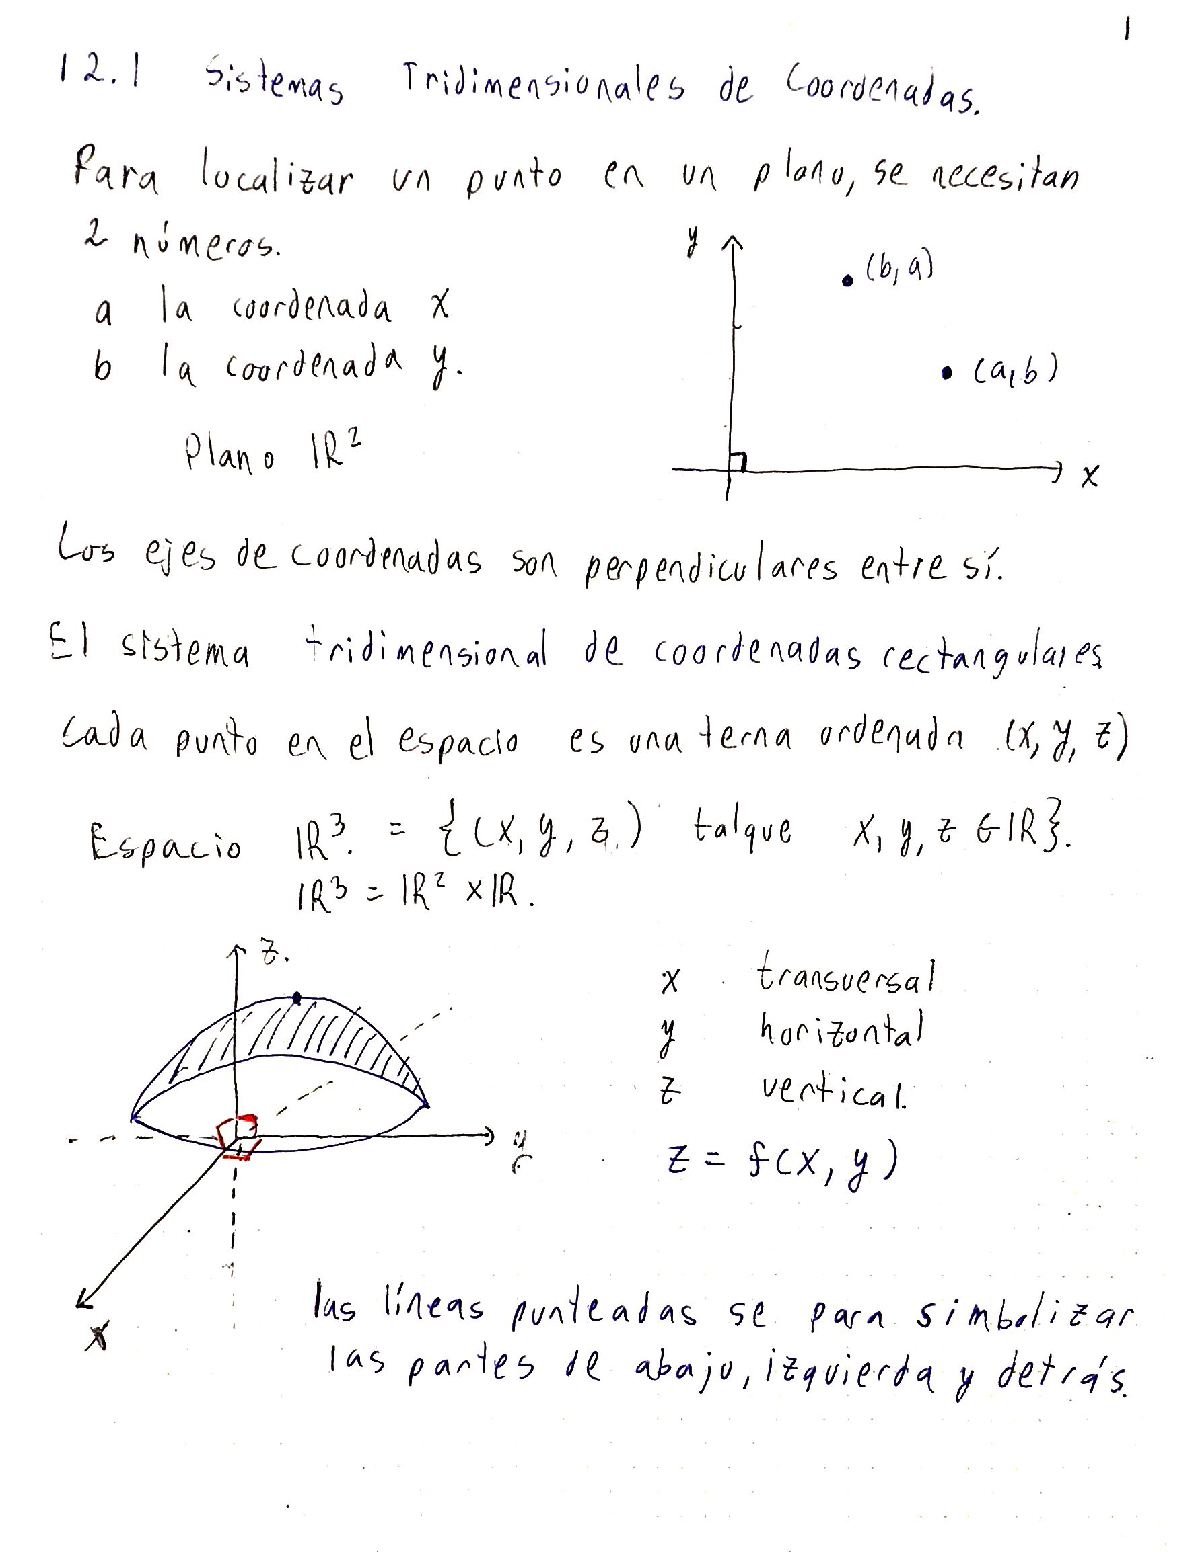
\includepdf[pages=-,pagecommand={\thispagestyle{plain}}]{\detokenize{RB/RB_2020-01-07_18_49_53.pdf}}


%%%%%%%%%%%%%%%%%%%%%%%%%%%%%%%%%%%%%%%%%%%%%%%%%%%%%%%%%%%%%%%%%%%%%%%%%%%%%%%%%%%%%%%%%%%%%%%%

\chapter{ Distancias y superficies básicas }
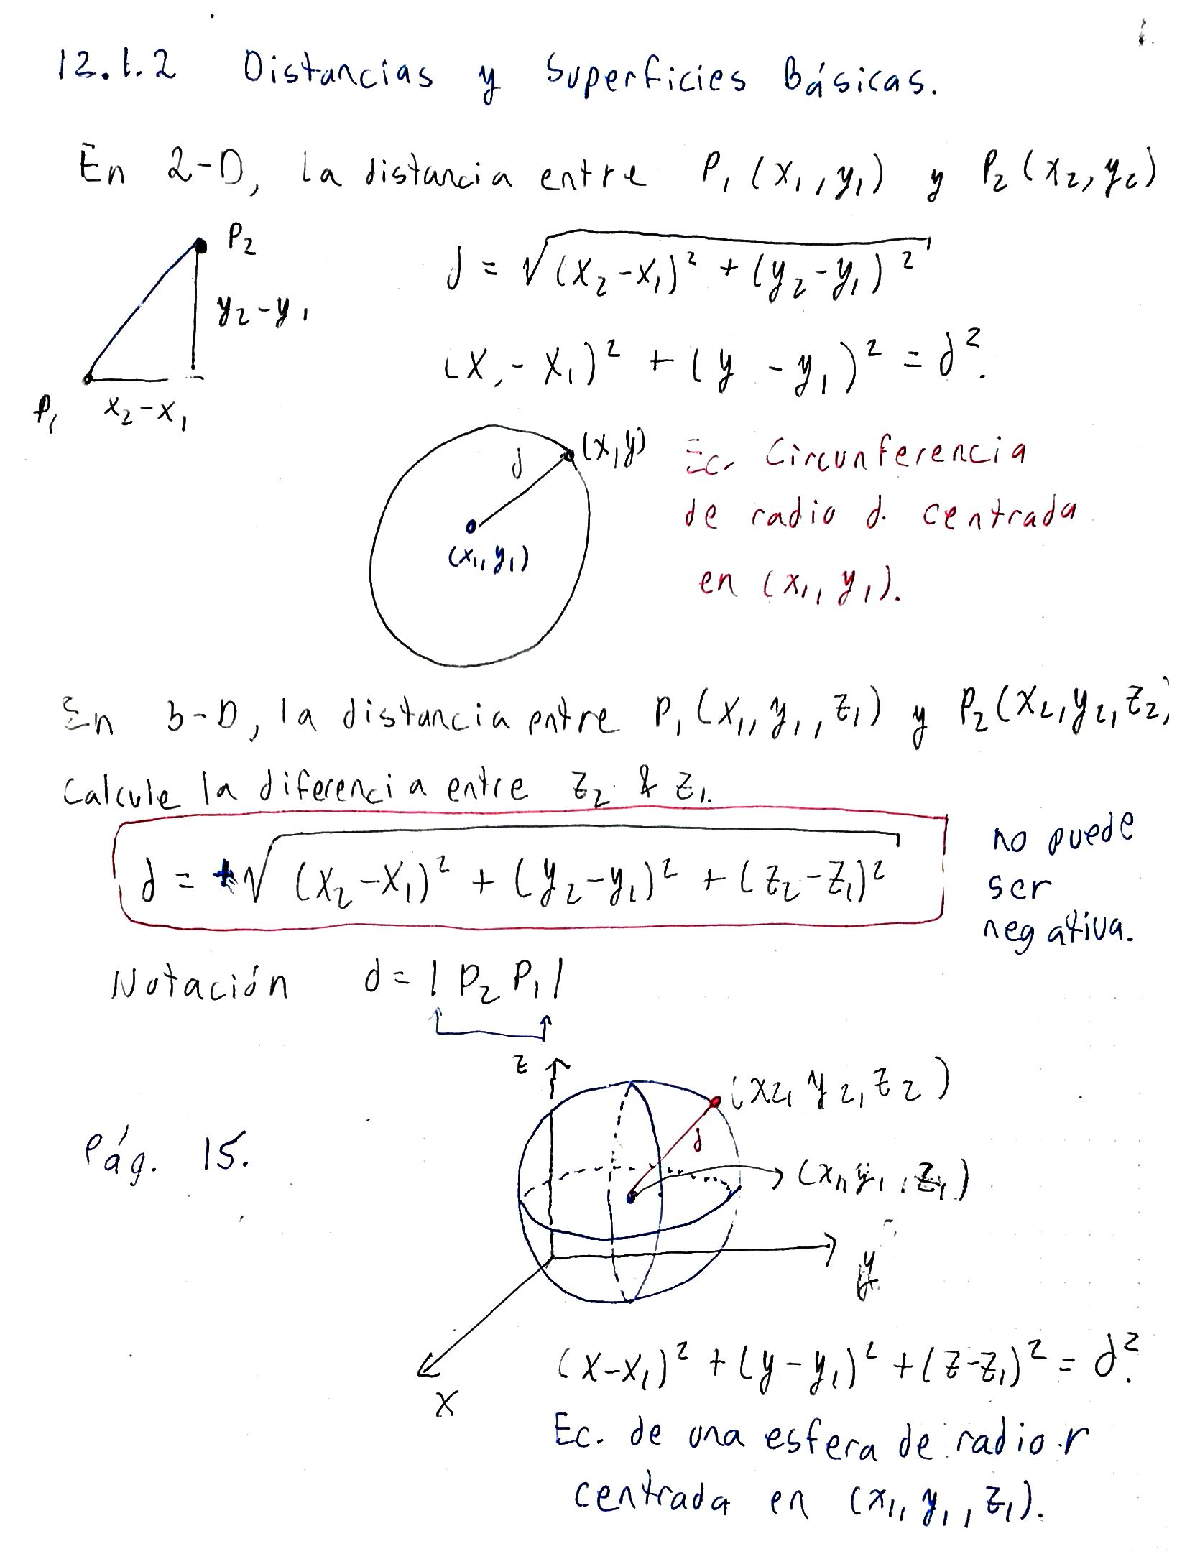
\includepdf[pages=-,pagecommand={\thispagestyle{plain}}]{\detokenize{RB/RB_2020-01-09_09_42_27.pdf}}


%%%%%%%%%%%%%%%%%%%%%%%%%%%%%%%%%%%%%%%%%%%%%%%%%%%%%%%%%%%%%%%%%%%%%%%%%%%%%%%%%%%%%%%%%%%%%%%%

\chapter{ Vectores }
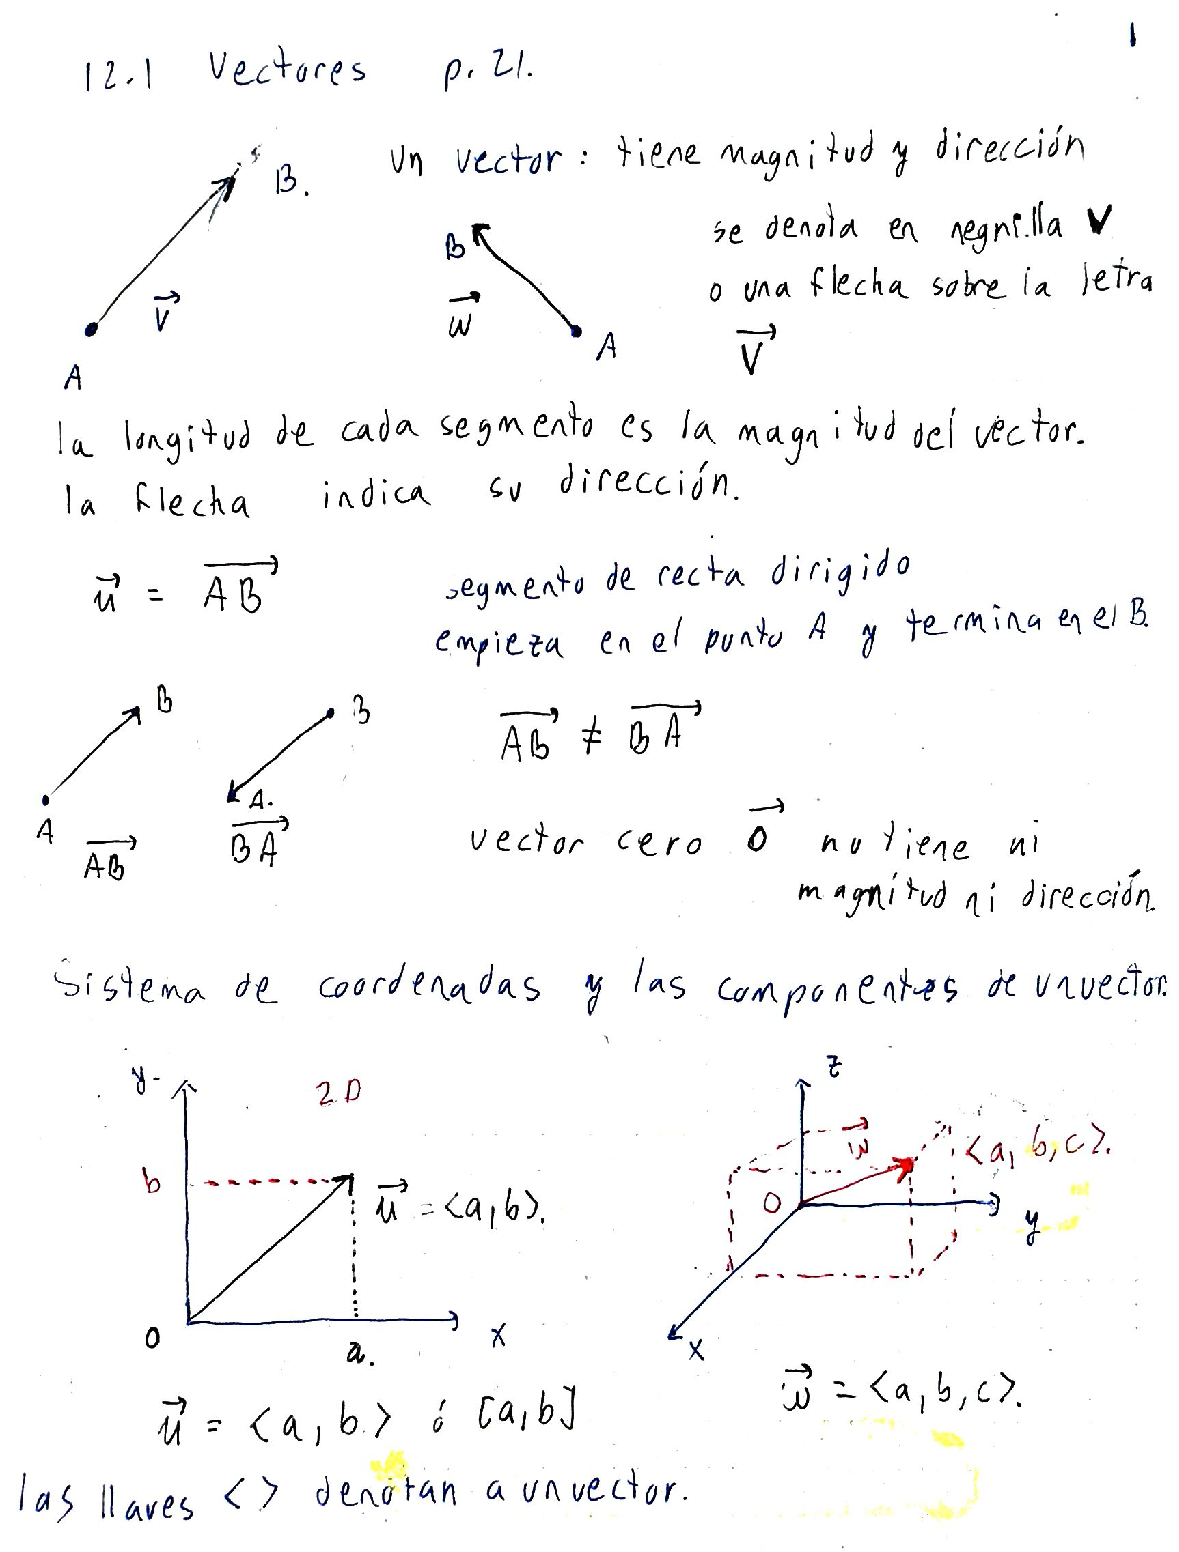
\includepdf[pages=-,pagecommand={\thispagestyle{plain}}]{\detokenize{RB/RB_2020-01-14_11_51_58.pdf}}


%%%%%%%%%%%%%%%%%%%%%%%%%%%%%%%%%%%%%%%%%%%%%%%%%%%%%%%%%%%%%%%%%%%%%%%%%%%%%%%%%%%%%%%%%%%%%%%%

\chapter{ Producto punto }
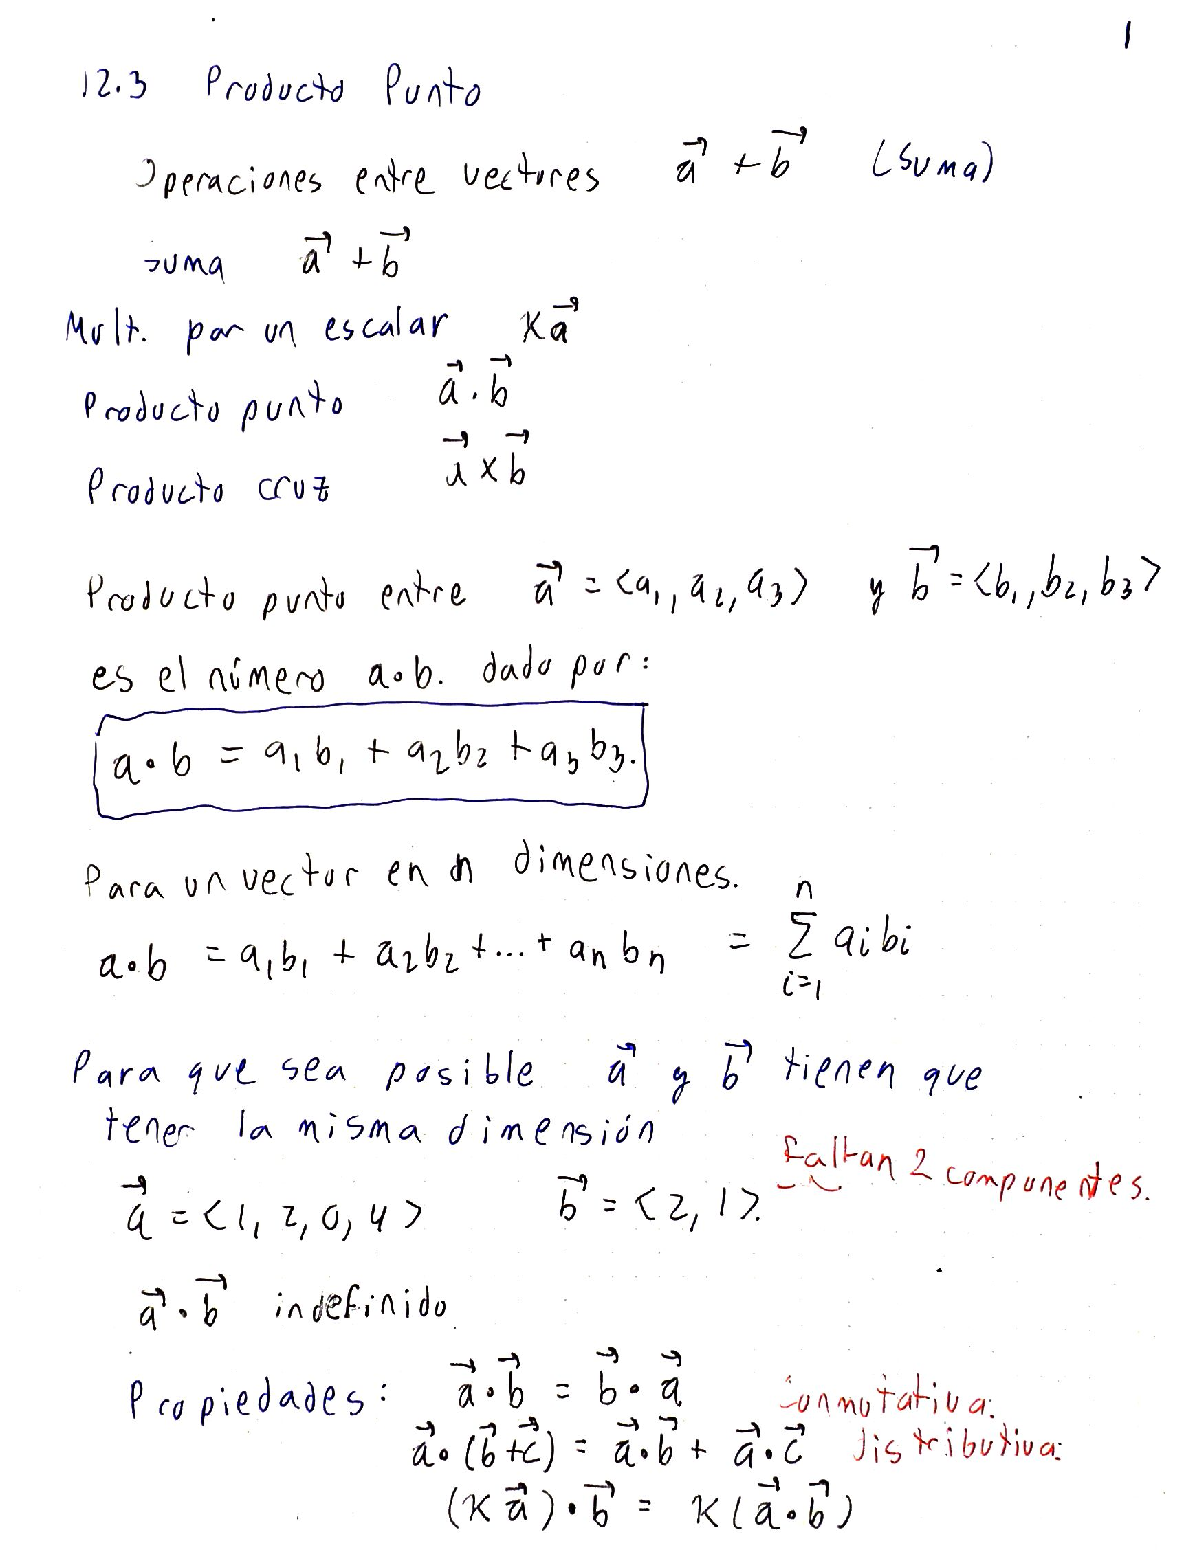
\includepdf[pages=-,pagecommand={\thispagestyle{plain}}]{\detokenize{RB/RB_2020-01-16_13_01_32.pdf}}


%%%%%%%%%%%%%%%%%%%%%%%%%%%%%%%%%%%%%%%%%%%%%%%%%%%%%%%%%%%%%%%%%%%%%%%%%%%%%%%%%%%%%%%%%%%%%%%%

\chapter{ Producto cruz }
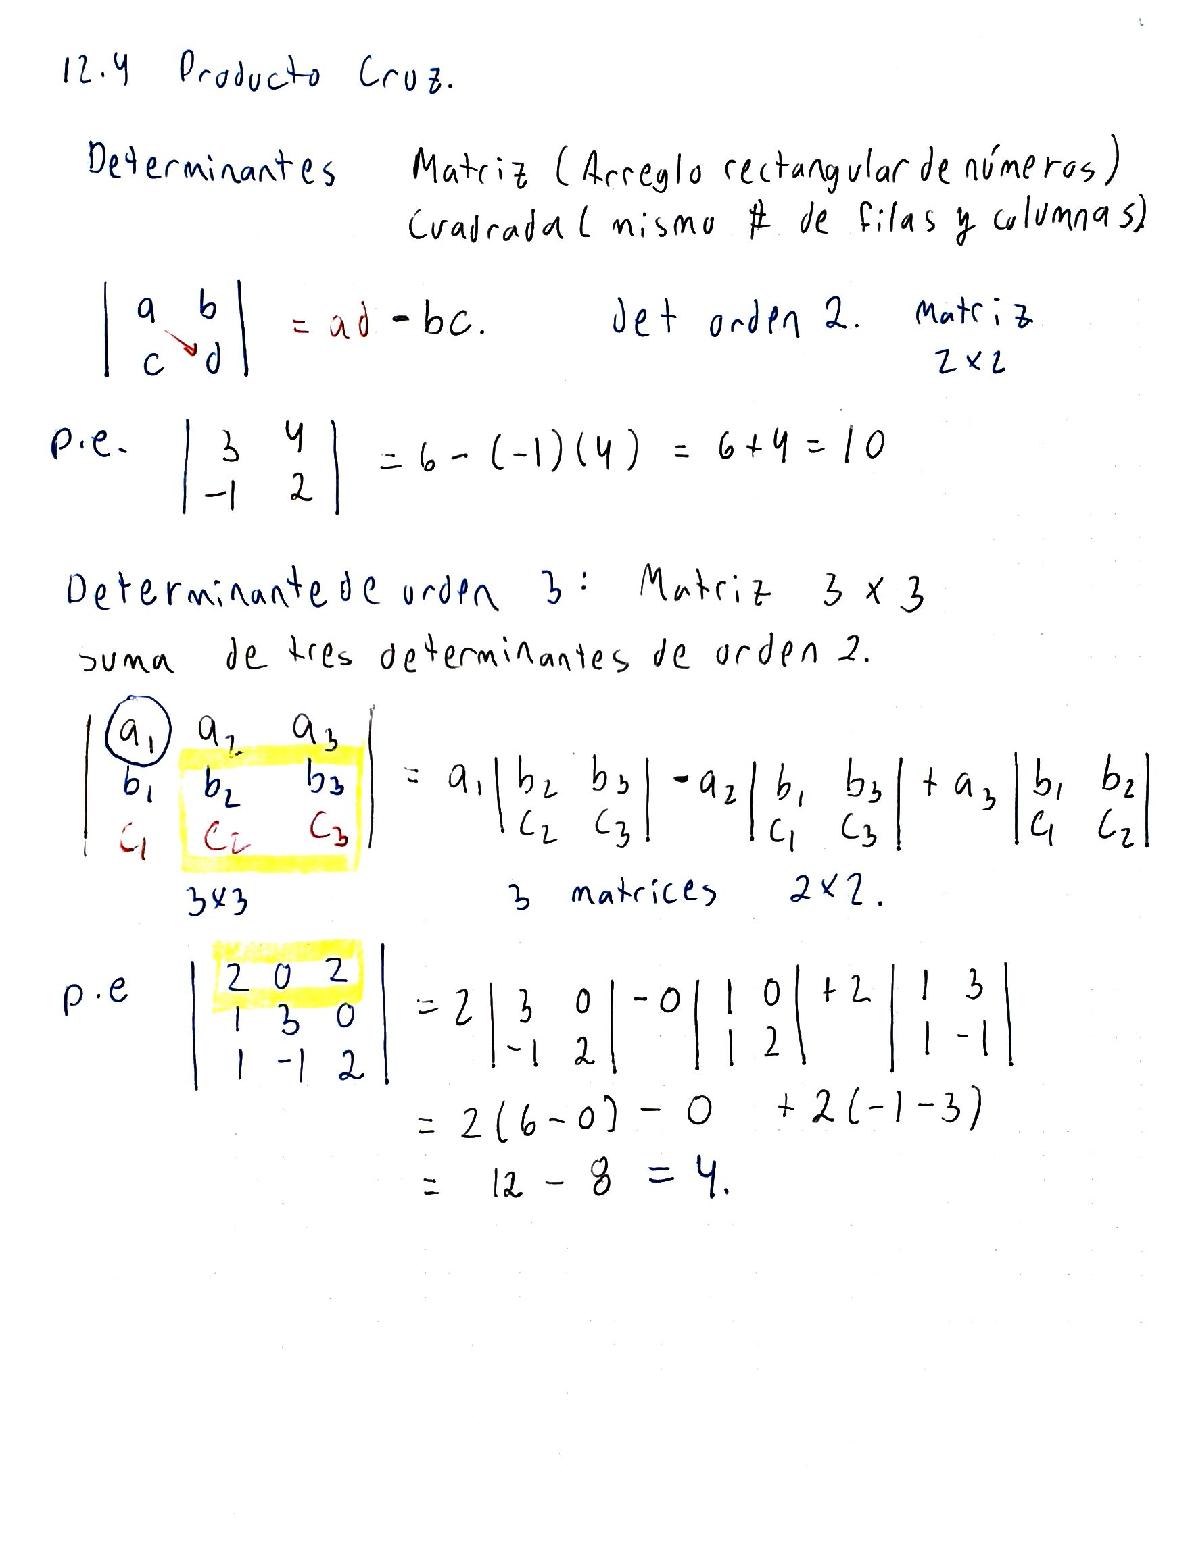
\includepdf[pages=-,pagecommand={\thispagestyle{plain}}]{\detokenize{RB/RB_2020-01-21_13_21_32.pdf}}


%%%%%%%%%%%%%%%%%%%%%%%%%%%%%%%%%%%%%%%%%%%%%%%%%%%%%%%%%%%%%%%%%%%%%%%%%%%%%%%%%%%%%%%%%%%%%%%%

\chapter{ Ángulo entre cetores y ejes \& Vectores paralelos y perpendiculares en n-dimensiones, Ecuación vectorial de una recta  }
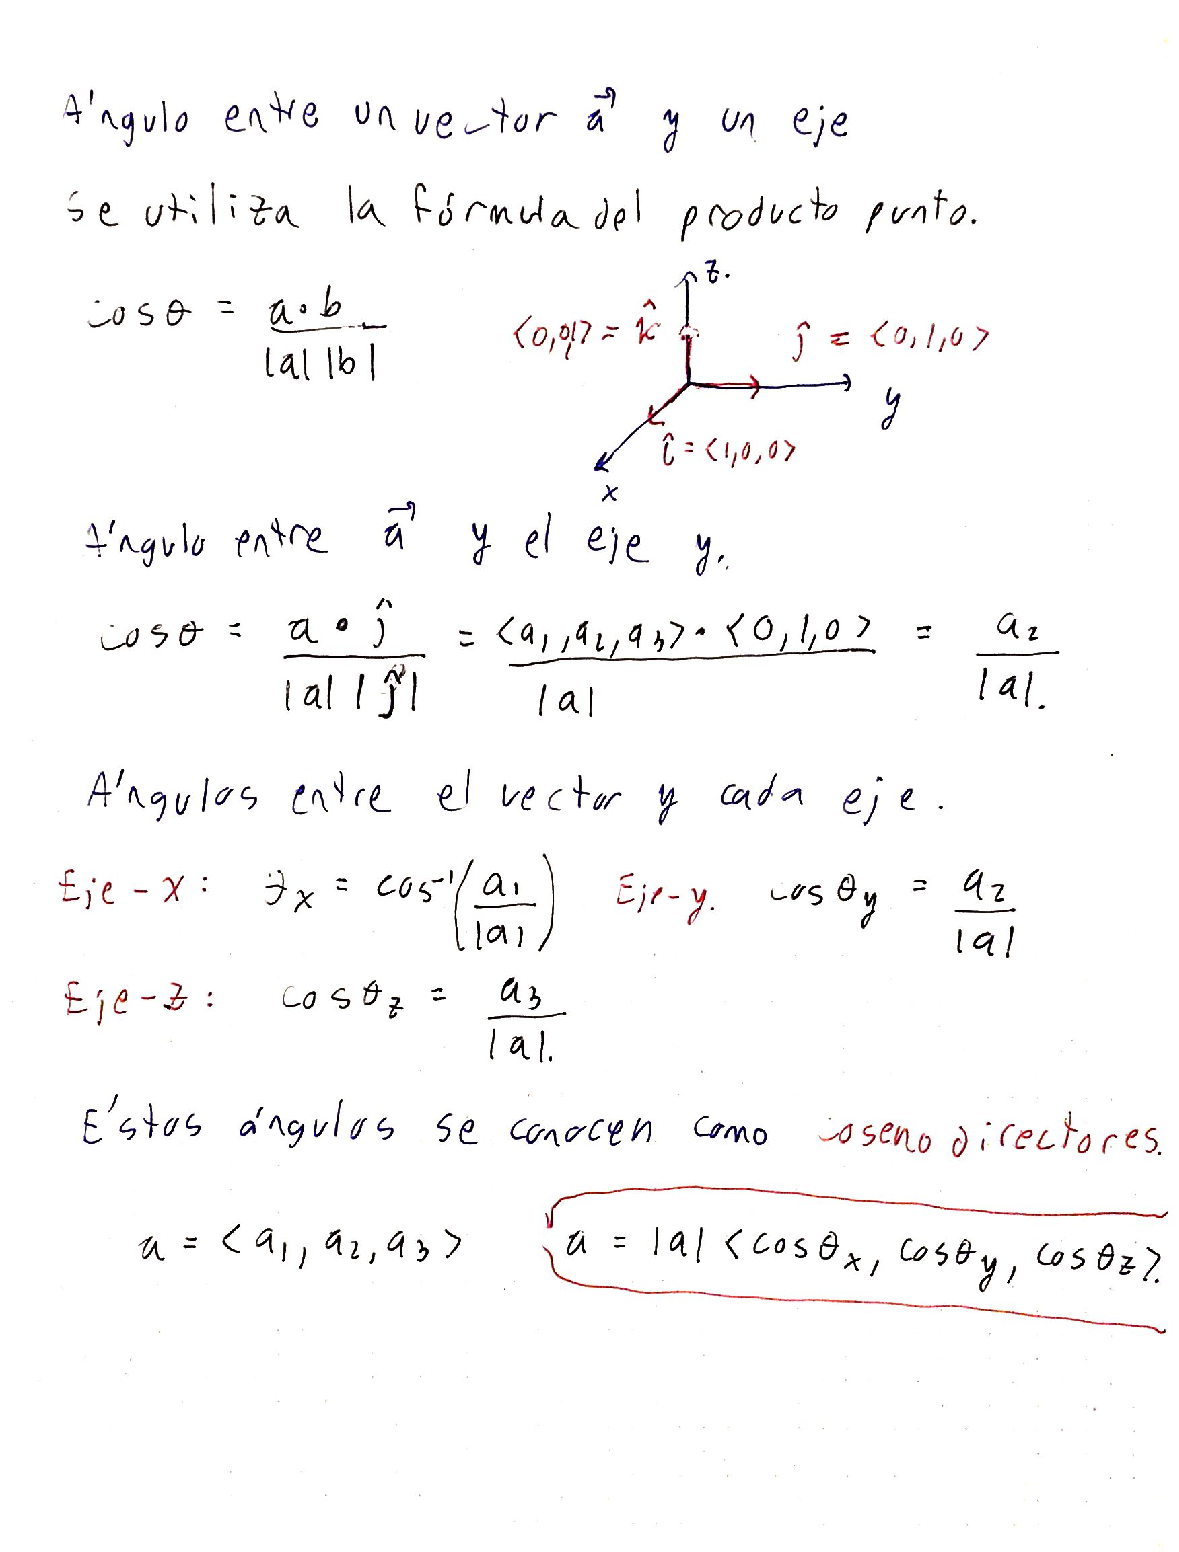
\includepdf[pages=-,pagecommand={\thispagestyle{plain}}]{\detokenize{RB/RB_2020-01-23_19_42_58.pdf}}


%%%%%%%%%%%%%%%%%%%%%%%%%%%%%%%%%%%%%%%%%%%%%%%%%%%%%%%%%%%%%%%%%%%%%%%%%%%%%%%%%%%%%%%%%%%%%%%%

\chapter{ Rectas y planos }
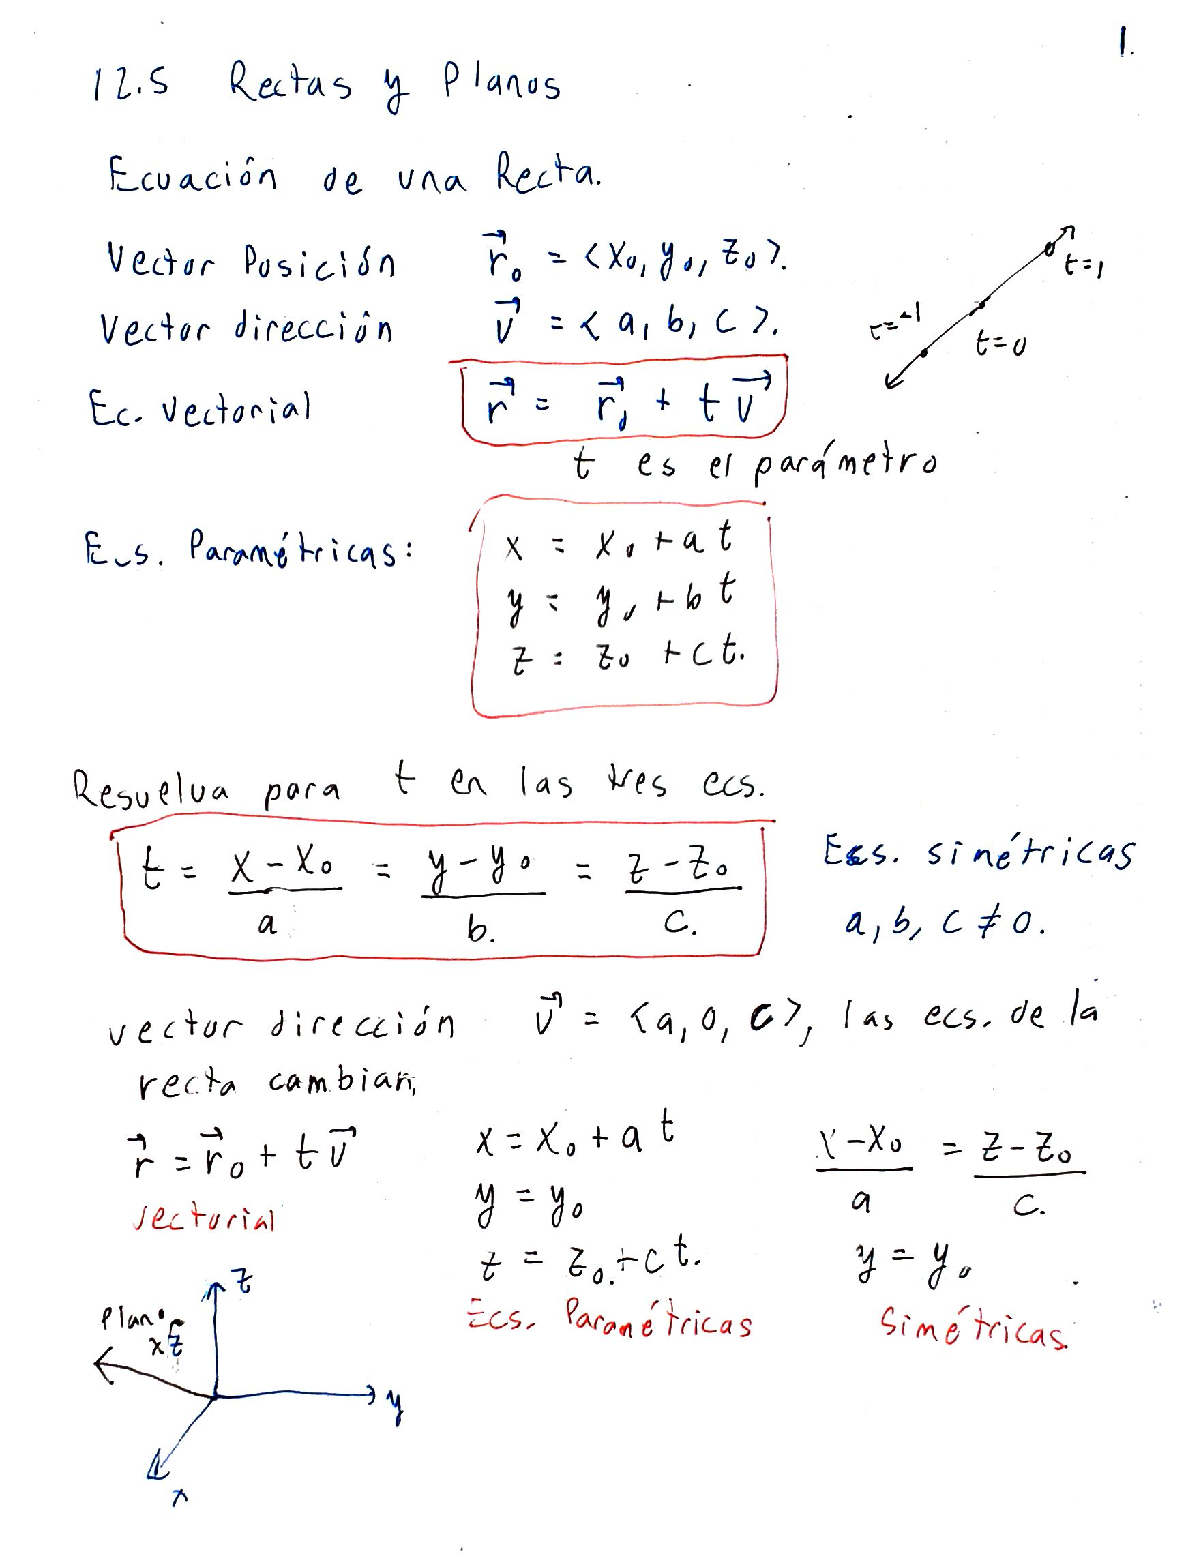
\includepdf[pages=-,pagecommand={\thispagestyle{plain}}]{\detokenize{RB/RB_2020-01-28_13_10_15.pdf}}


%%%%%%%%%%%%%%%%%%%%%%%%%%%%%%%%%%%%%%%%%%%%%%%%%%%%%%%%%%%%%%%%%%%%%%%%%%%%%%%%%%%%%%%%%%%%%%%%

\chapter{ Continuación de rectas y planos }
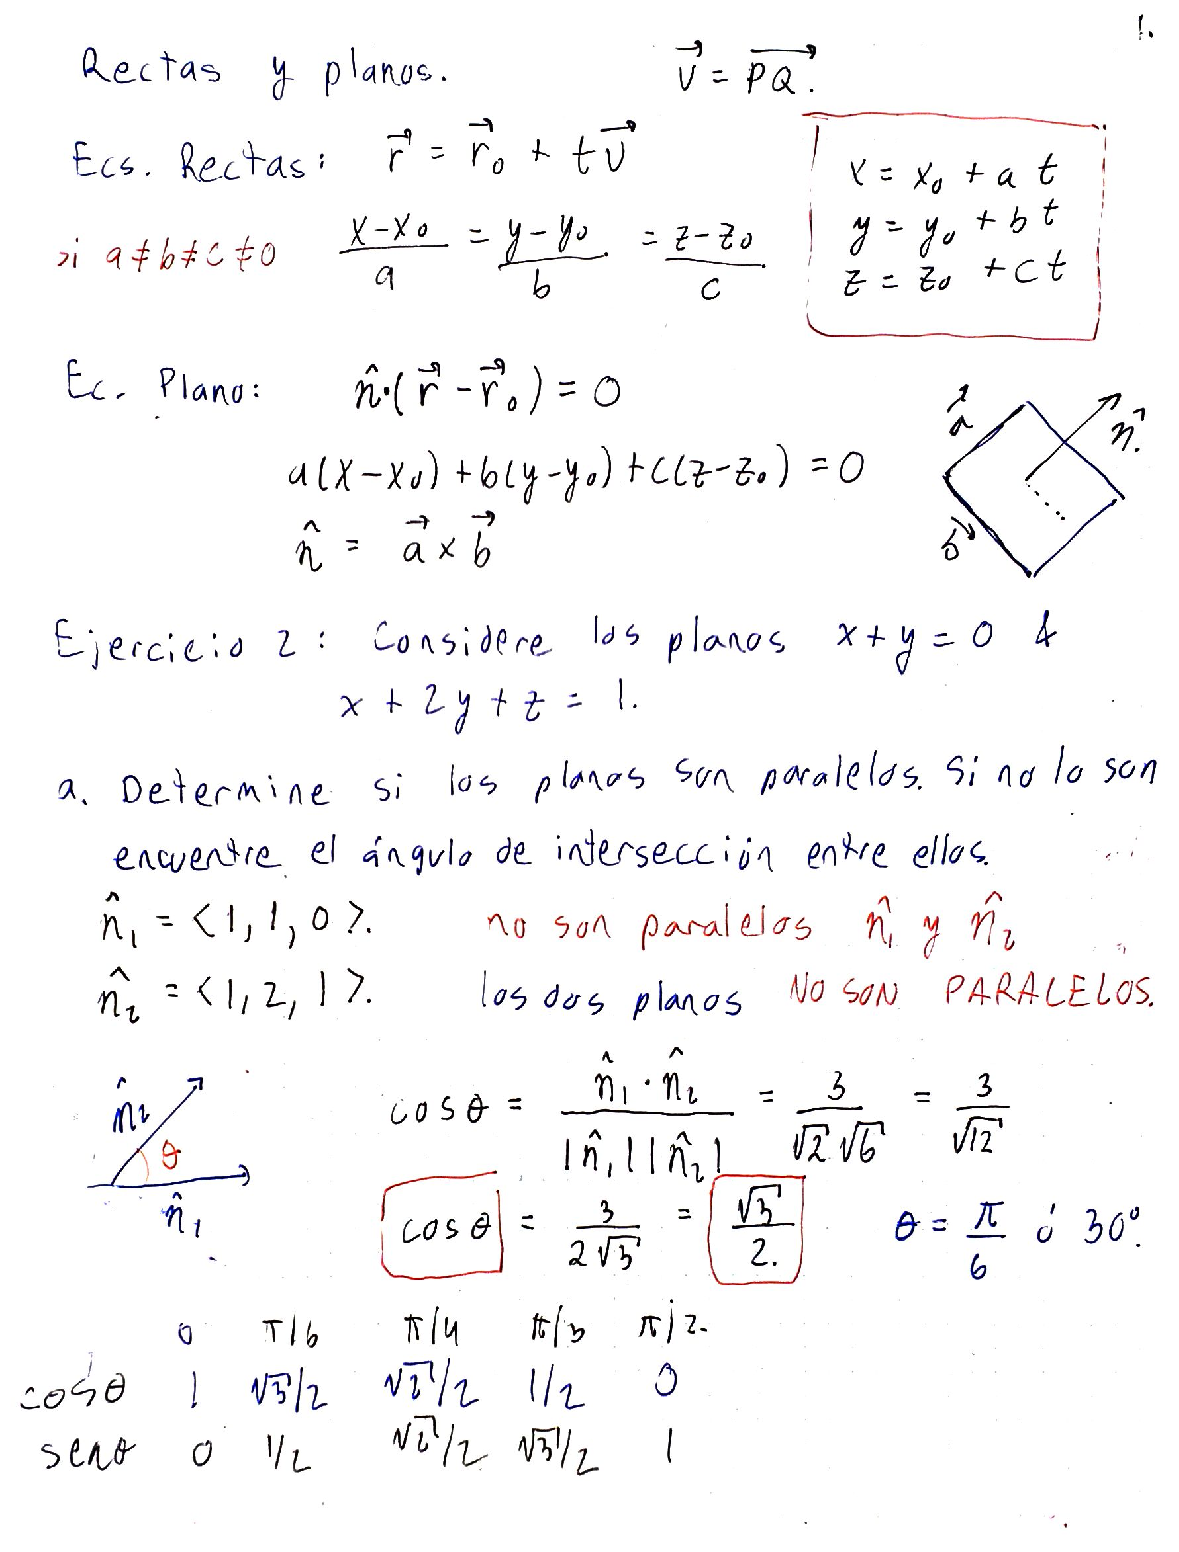
\includepdf[pages=-,pagecommand={\thispagestyle{plain}}]{\detokenize{RB/RB_2020-01-30_11_31_17.pdf}}


%%%%%%%%%%%%%%%%%%%%%%%%%%%%%%%%%%%%%%%%%%%%%%%%%%%%%%%%%%%%%%%%%%%%%%%%%%%%%%%%%%%%%%%%%%%%%%%%

\chapter{ Funciones Vectoriales \& Límites y continuidad }
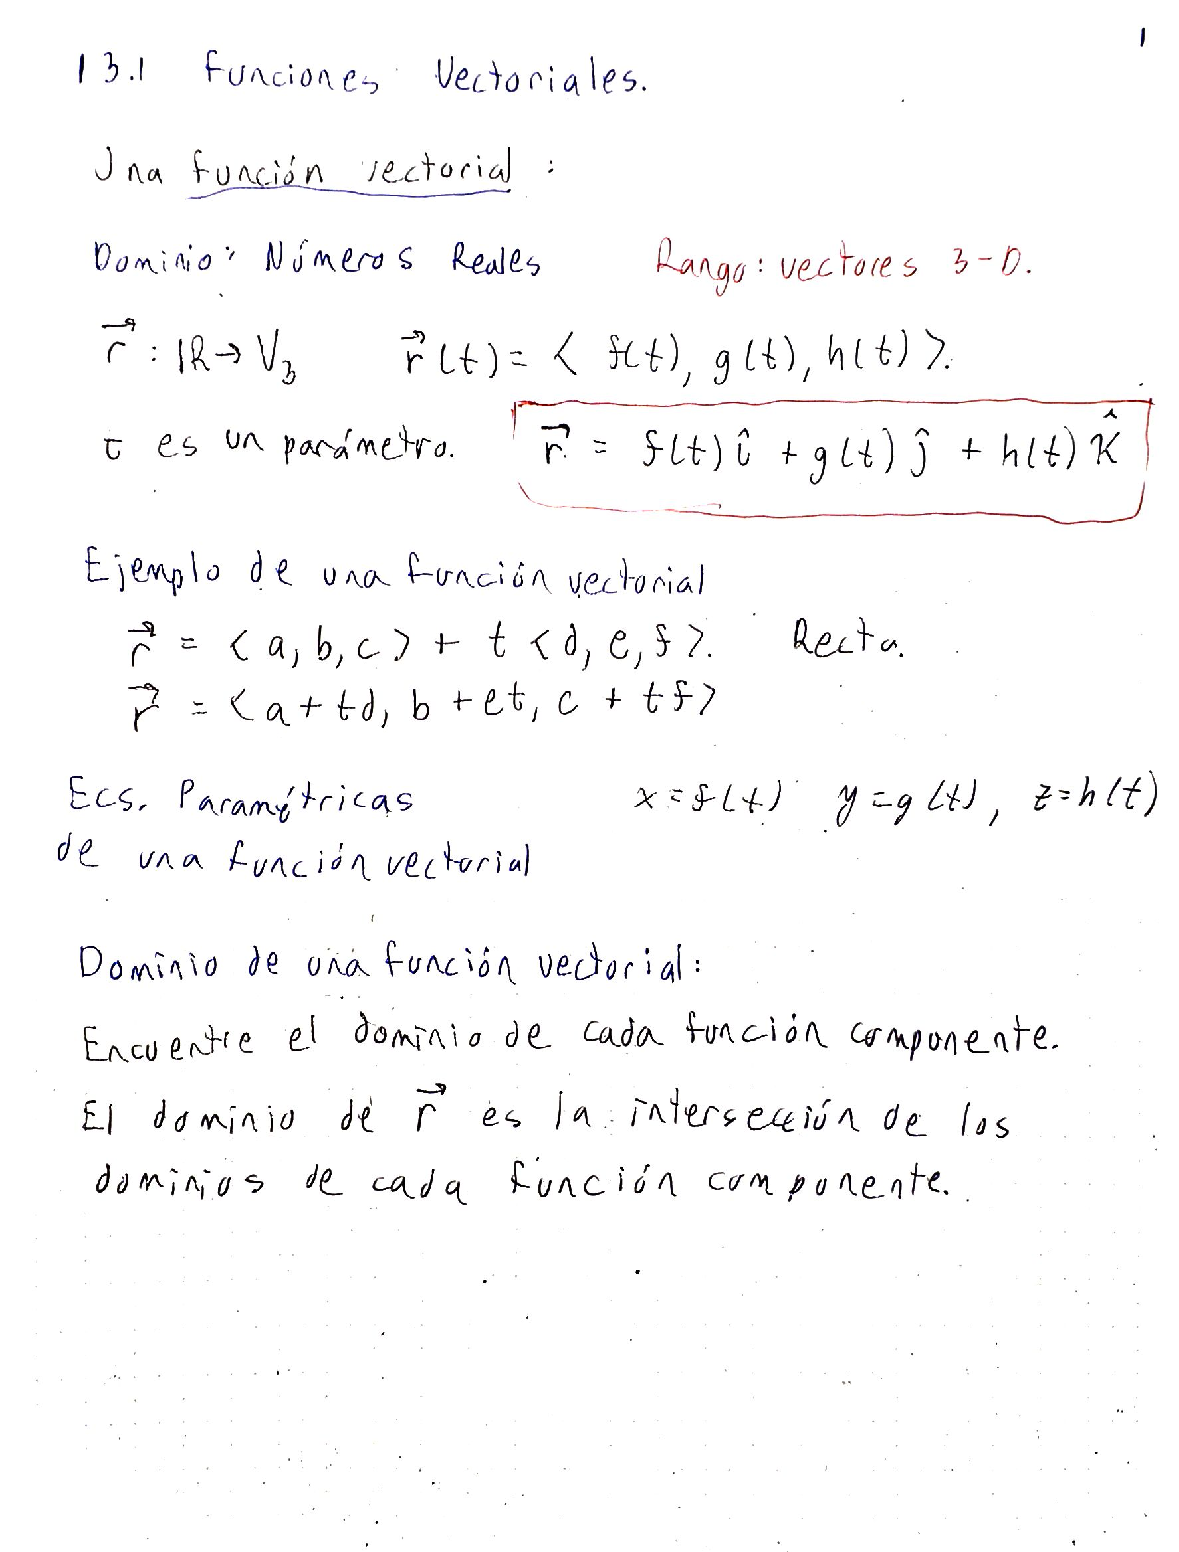
\includepdf[pages=-,pagecommand={\thispagestyle{plain}}]{\detokenize{RB/RB_2020-02-04_11_22_59.pdf}}


%%%%%%%%%%%%%%%%%%%%%%%%%%%%%%%%%%%%%%%%%%%%%%%%%%%%%%%%%%%%%%%%%%%%%%%%%%%%%%%%%%%%%%%%%%%%%%%%

\chapter{ Cálculo con funciones vectoriales: derivadas, integrales, etcétera }
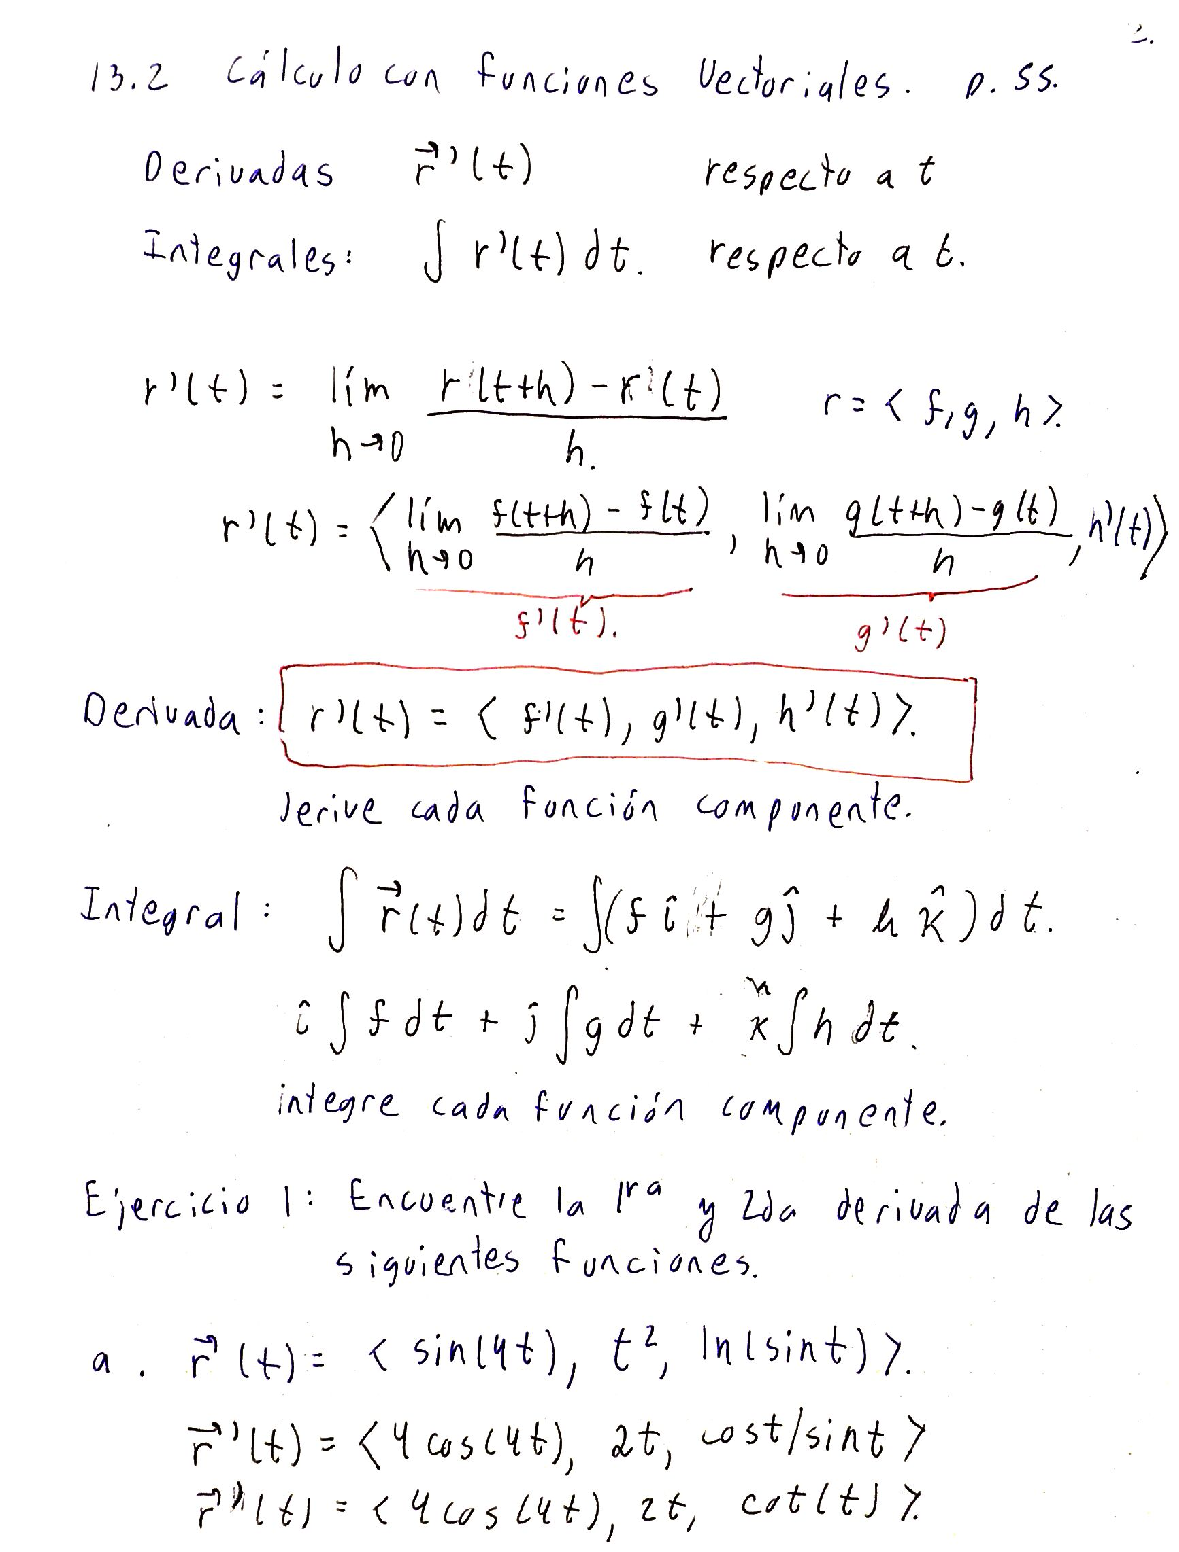
\includepdf[pages=-,pagecommand={\thispagestyle{plain}}]{\detokenize{RB/RB_2020-02-06_10_19_48.pdf}}


%%%%%%%%%%%%%%%%%%%%%%%%%%%%%%%%%%%%%%%%%%%%%%%%%%%%%%%%%%%%%%%%%%%%%%%%%%%%%%%%%%%%%%%%%%%%%%%%

\chapter{ Continuación de cálculo con funciones vectoriales }
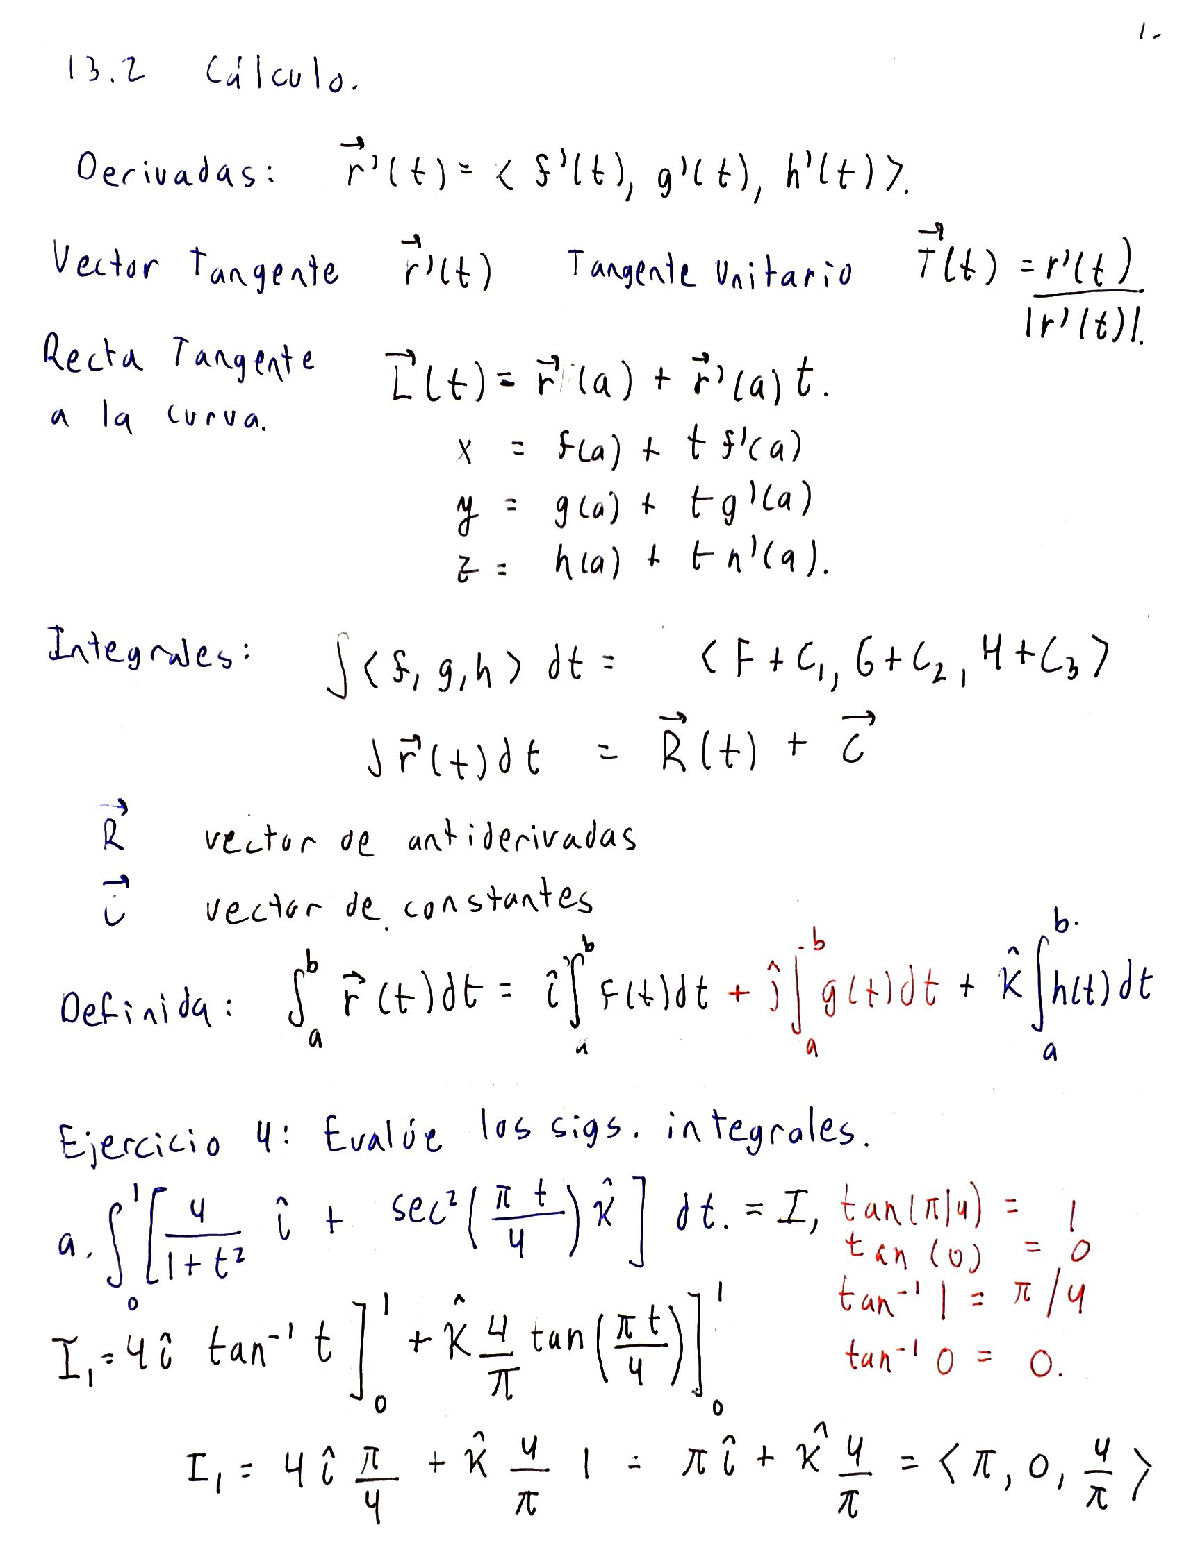
\includepdf[pages=-,pagecommand={\thispagestyle{plain}}]{\detokenize{RB/RB_2020-02-11_13_33_43.pdf}}


%%%%%%%%%%%%%%%%%%%%%%%%%%%%%%%%%%%%%%%%%%%%%%%%%%%%%%%%%%%%%%%%%%%%%%%%%%%%%%%%%%%%%%%%%%%%%%%%

\chapter{ Funciones de varias variables }
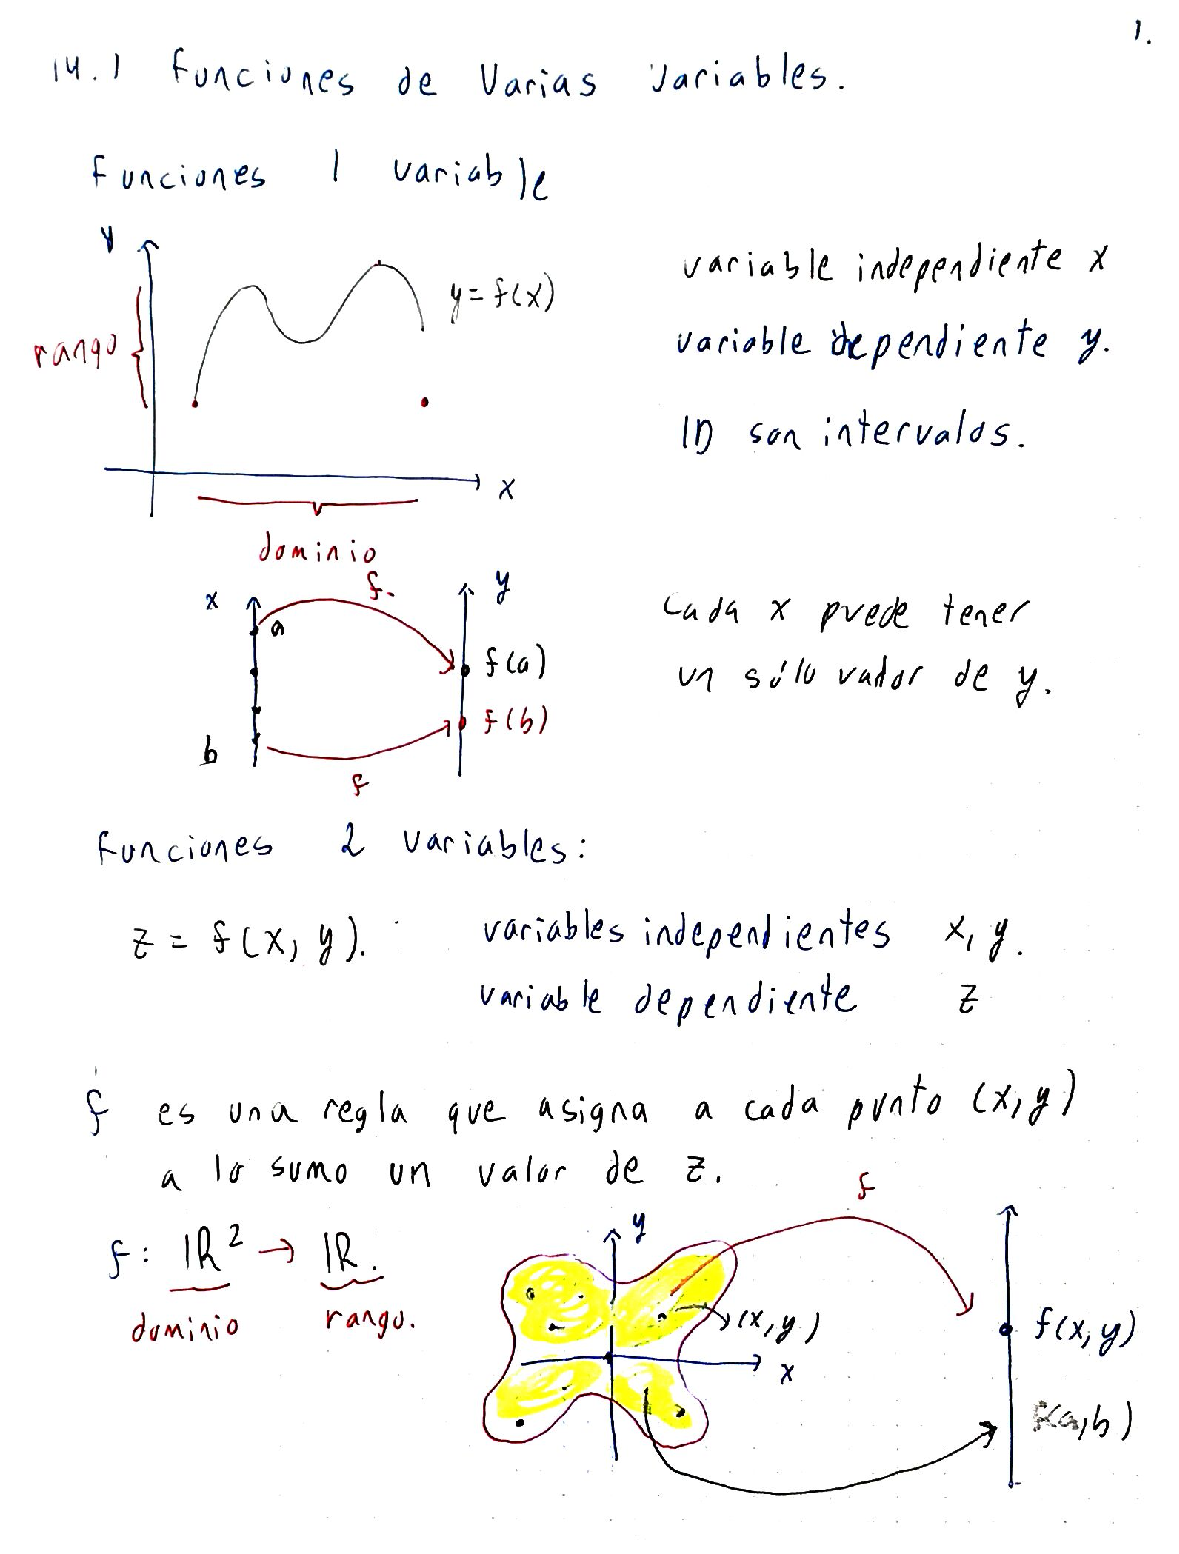
\includepdf[pages=-,pagecommand={\thispagestyle{plain}}]{\detokenize{RB/RB_2020-02-14_08_56_40.pdf}}


%%%%%%%%%%%%%%%%%%%%%%%%%%%%%%%%%%%%%%%%%%%%%%%%%%%%%%%%%%%%%%%%%%%%%%%%%%%%%%%%%%%%%%%%%%%%%%%%

\chapter{ Curvas de nivel }
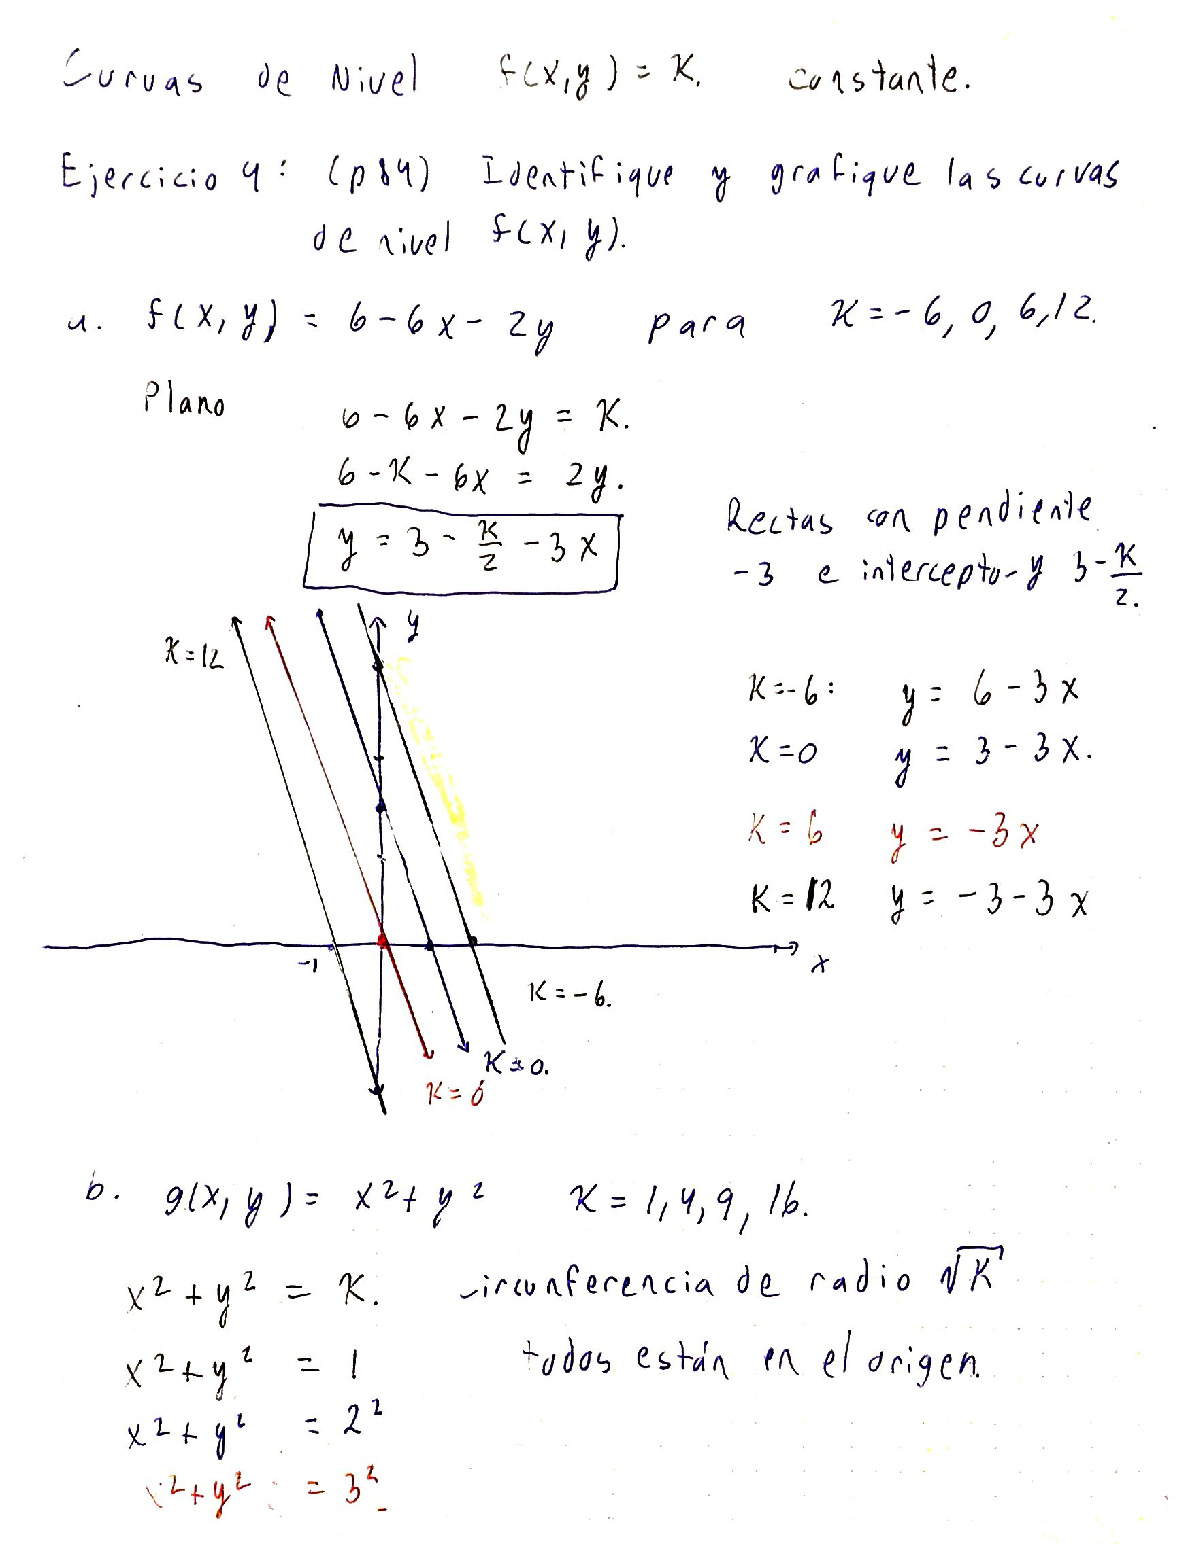
\includepdf[pages=-,pagecommand={\thispagestyle{plain}}]{\detokenize{RB/RB_2020-02-18_10_21_11.pdf}}


%%%%%%%%%%%%%%%%%%%%%%%%%%%%%%%%%%%%%%%%%%%%%%%%%%%%%%%%%%%%%%%%%%%%%%%%%%%%%%%%%%%%%%%%%%%%%%%%

\chapter{ Derivadas parciales }
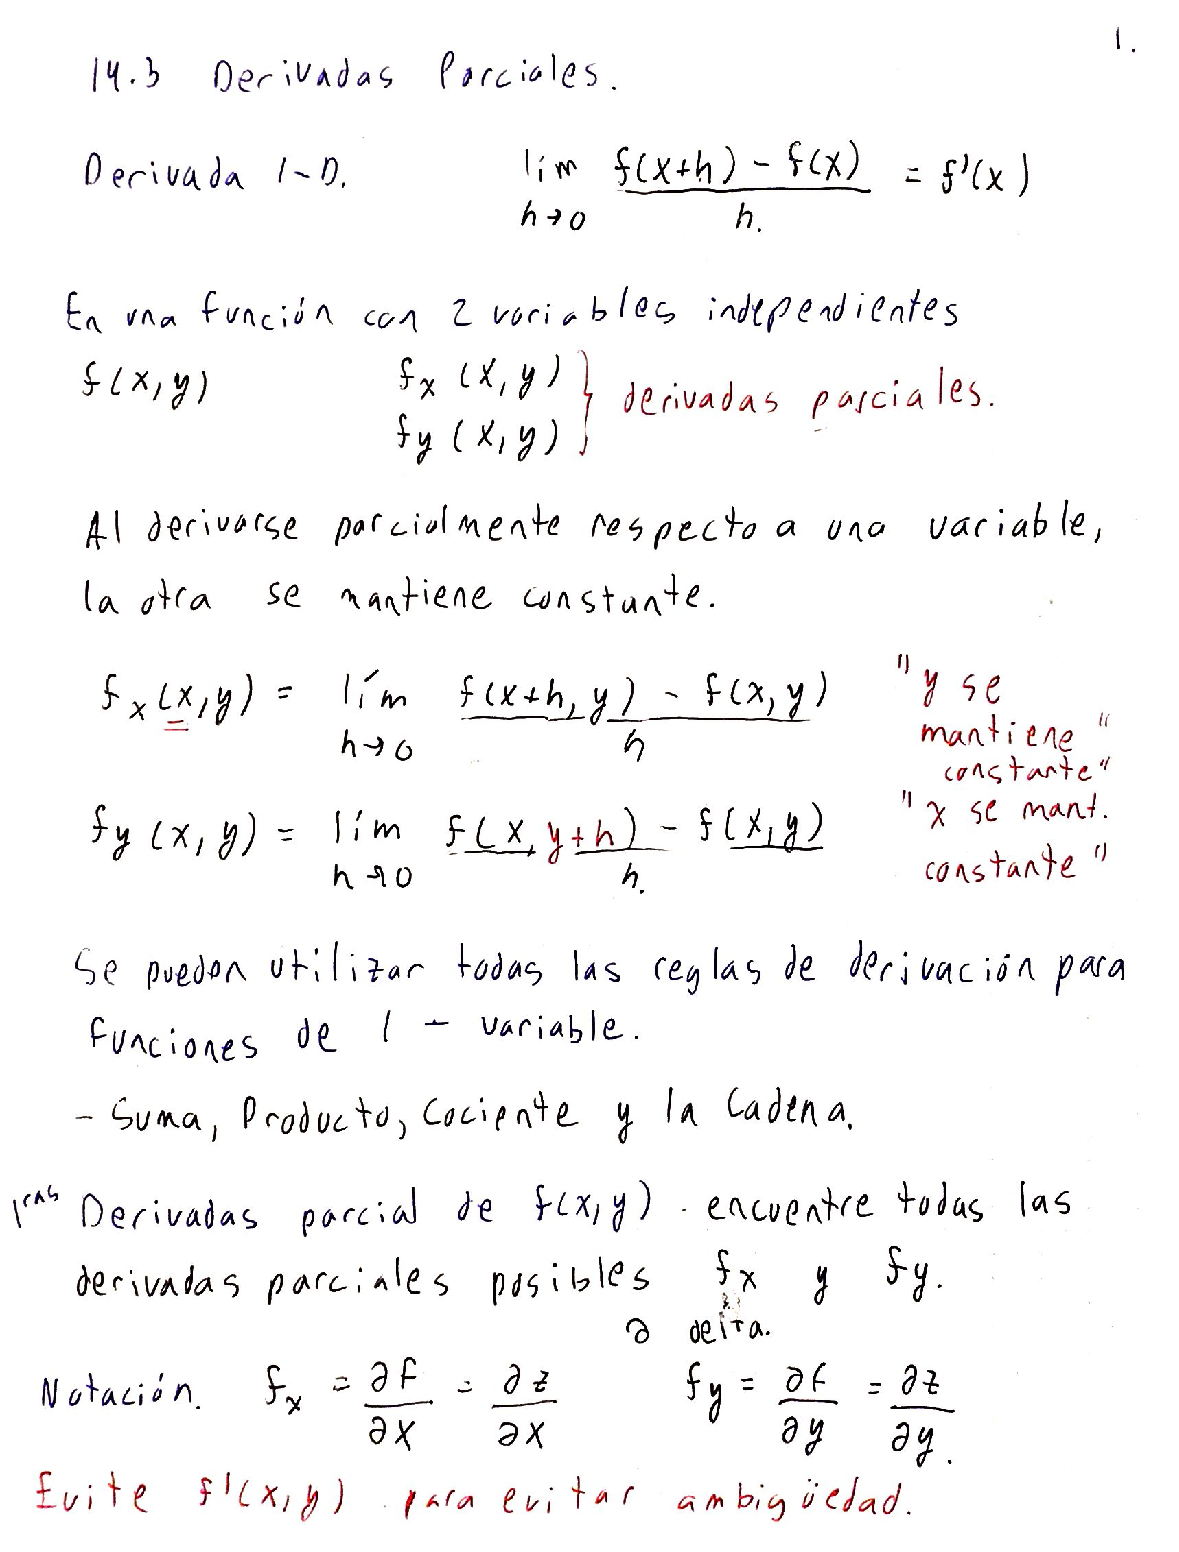
\includepdf[pages=-,pagecommand={\thispagestyle{plain}}]{\detokenize{RB/RB_2020-02-20_10_58_23.pdf}}


%%%%%%%%%%%%%%%%%%%%%%%%%%%%%%%%%%%%%%%%%%%%%%%%%%%%%%%%%%%%%%%%%%%%%%%%%%%%%%%%%%%%%%%%%%%%%%%%

\chapter{ Derivadas parciales, rectas tangentes y planos tangentes }
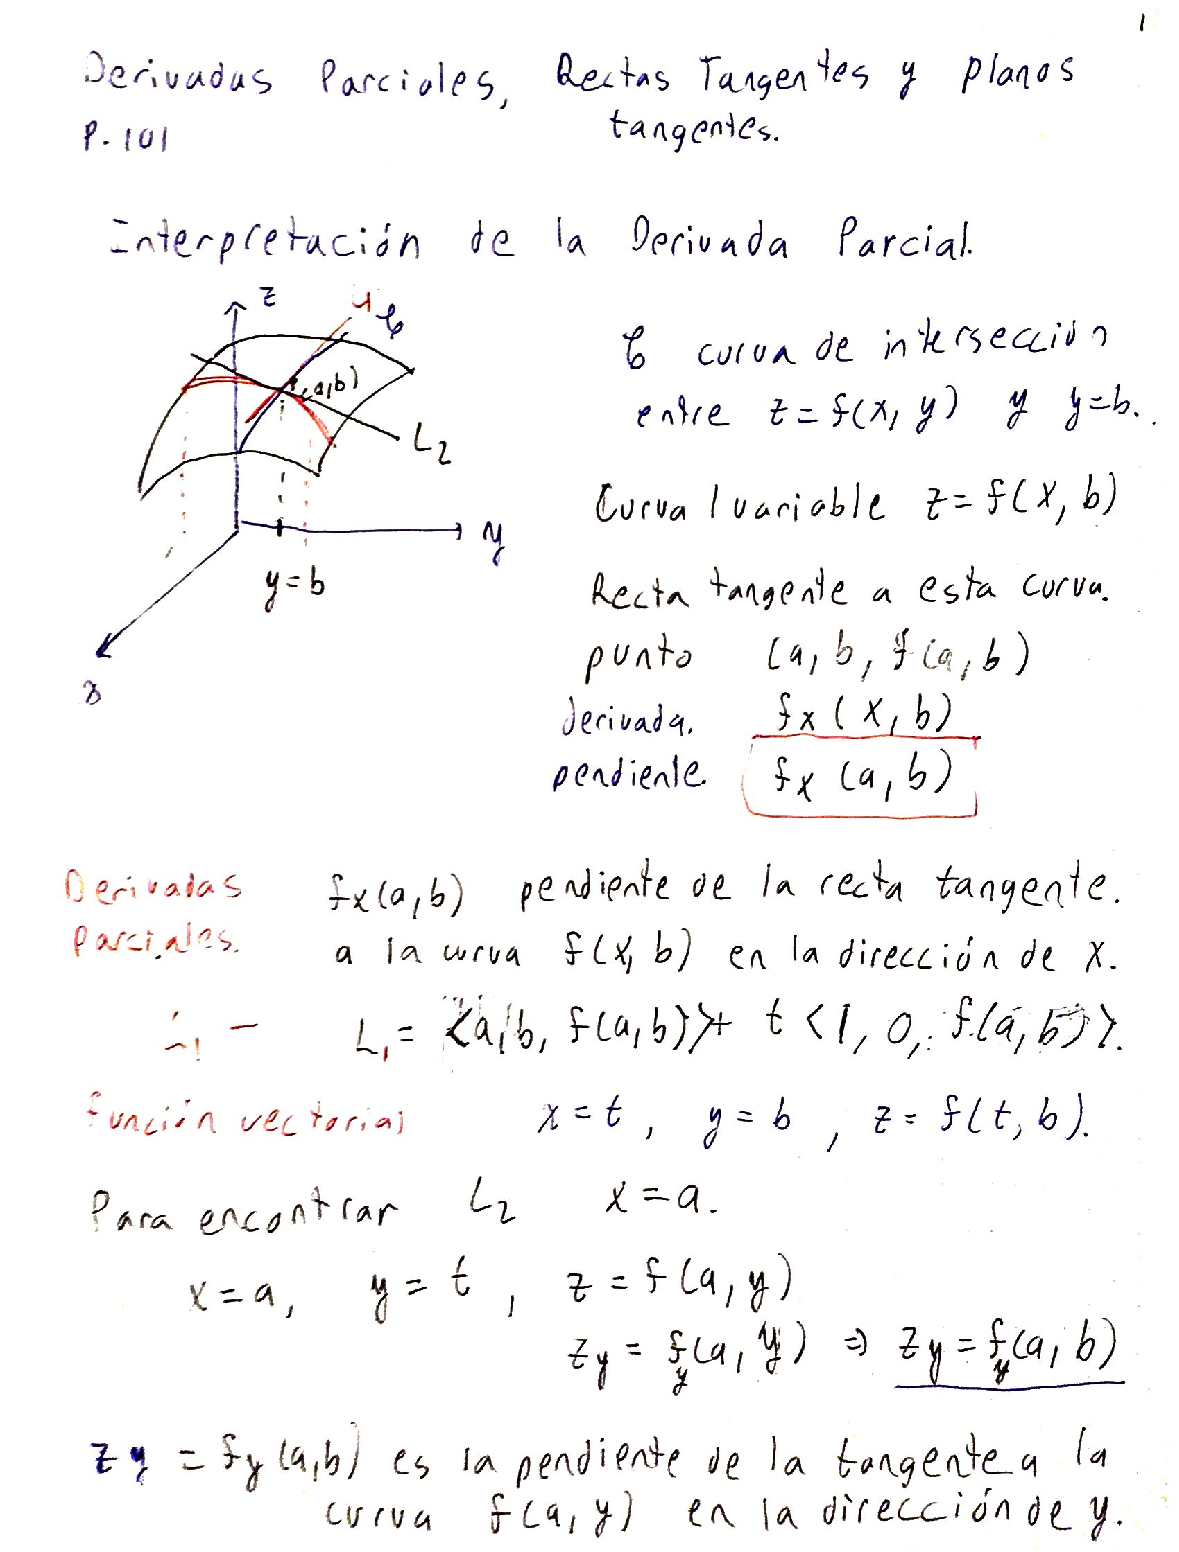
\includepdf[pages=-,pagecommand={\thispagestyle{plain}}]{\detokenize{RB/RB_2020-02-27_10_04_55.pdf}}


%%%%%%%%%%%%%%%%%%%%%%%%%%%%%%%%%%%%%%%%%%%%%%%%%%%%%%%%%%%%%%%%%%%%%%%%%%%%%%%%%%%%%%%%%%%%%%%%

\end{document}
